
%(BEGIN_QUESTION)
% Copyright 2010, Tony R. Kuphaldt, released under the Creative Commons Attribution License (v 1.0)
% This means you may do almost anything with this work of mine, so long as you give me proper credit

Connect an oscilloscope in parallel with the VFD's power line connections (through a step-down transformer) to monitor the input voltage waveform while the drive is running and while it is stopped.  What effect do you notice on the sine wave's shape when the drive is active?

Try sketching each waveshape (drive running vs. not running) here:

$$\includegraphics[width=15.5cm]{i04065x01.eps}$$

\vskip 10pt

Another experiment to try is operating an AM radio near a VFD when it is stopped versus when it is running.  Explain why the radio responds as it does to the VFD's status.

\vskip 20pt \vbox{\hrule \hbox{\strut \vrule{} {\bf Suggestions for Socratic discussion} \vrule} \hrule}

\begin{itemize}
\item{} How might the harmonics generated by a VFD interfere with nearby electronic equipment?
\item{} How can a technician detect the presence of harmonics, and more importantly locate the precise source of harmonic distortion in a power system?
\item{} How is it possible to ``shield'' other equipment on the power system from harmonics generated by a particular VFD?
\end{itemize}


\underbar{file i04065}
%(END_QUESTION)





%(BEGIN_ANSWER)


%(END_ANSWER)





%(BEGIN_NOTES)

%INDEX% Final Control Elements, motor: variable frequency drive

%(END_NOTES)

